\documentclass[final]{beamer} % use beamer

%\usepackage[usenames,dvipsnames]{xcolor}
\usepackage[orientation=landscale,size=a0,scale=1.6]{beamerposter}
\usepackage[english]{babel}
\usepackage[utf8]{inputenc}
\usepackage{amsfonts}
\usepackage{amsthm}
\usepackage{amsmath}
\usepackage{pgf}
\usepackage{palatino}
\usepackage{comment}
\usepackage{natbib}
\usepackage{paralist}
\usepackage{epstopdf}
\usepackage{algorithm}
\usepackage{caption}
\usepackage{algorithmic}
\usepackage{tcolorbox}
\setbeamertemplate{bibliography item}[text]

\setlength{\leftmargini}{2cm}


%\usetheme{bpiresicml2013}
\usepackage{beamerthemebpiresicml2013}

%\setbeamercolor{block title}{fg=black,bg=white}
%\setbeamercolor{block body}{fg=black,bg=white}
%--set colors for alerted blocks (with frame)----------------------------------
%--textcolor = fg, backgroundcolor = bg, dblue is the jacobs blue
%\setbeamercolor{block alerted title}{fg=white,bg=uofagreen!70}%frame color
 %\setbeamercolor{block alerted body}{fg=black,bg=uofagreen!10}%body color

%==Title, date and authors of the poster=======================================

\newcommand{\eps}{\epsilon}
\DeclareMathOperator{\pol}{Poly}
\DeclareMathOperator{\real}{\mathbb{R}}
\newcommand{\poly}[1]{\pol\left(#1\right)}
\newcommand{\EEp}[1]{\mathbb{E}\left[#1\right]}
\newtheorem{thm}{Theorem}[section]

%\addtobeamertemplate{block begin}{}{\setlength{\parskip}{35pt plus 1pt minus 1pt}}

\title{Deterministic Independent Component Analysis (ICA)}
\author{Ruitong Huang, Andr\'as Gy\"orgy, Csaba Szepesv\'{a}ri}


\begin{document}

\begin{frame}[c]
	\vspace{-1.5cm}

	\begin{columns}[t,totalwidth=\textwidth]
	
	\begin{column}{0.01\textwidth}
	\end{column}
%------------------------------------------------------------------------------
% The first column
%------------------------------------------------------------------------------	

		
 	\begin{column}{.24\textwidth}% the right size for a 3-column layout
	
		\begin{block}{What is ICA?}
			\begin{figure}
				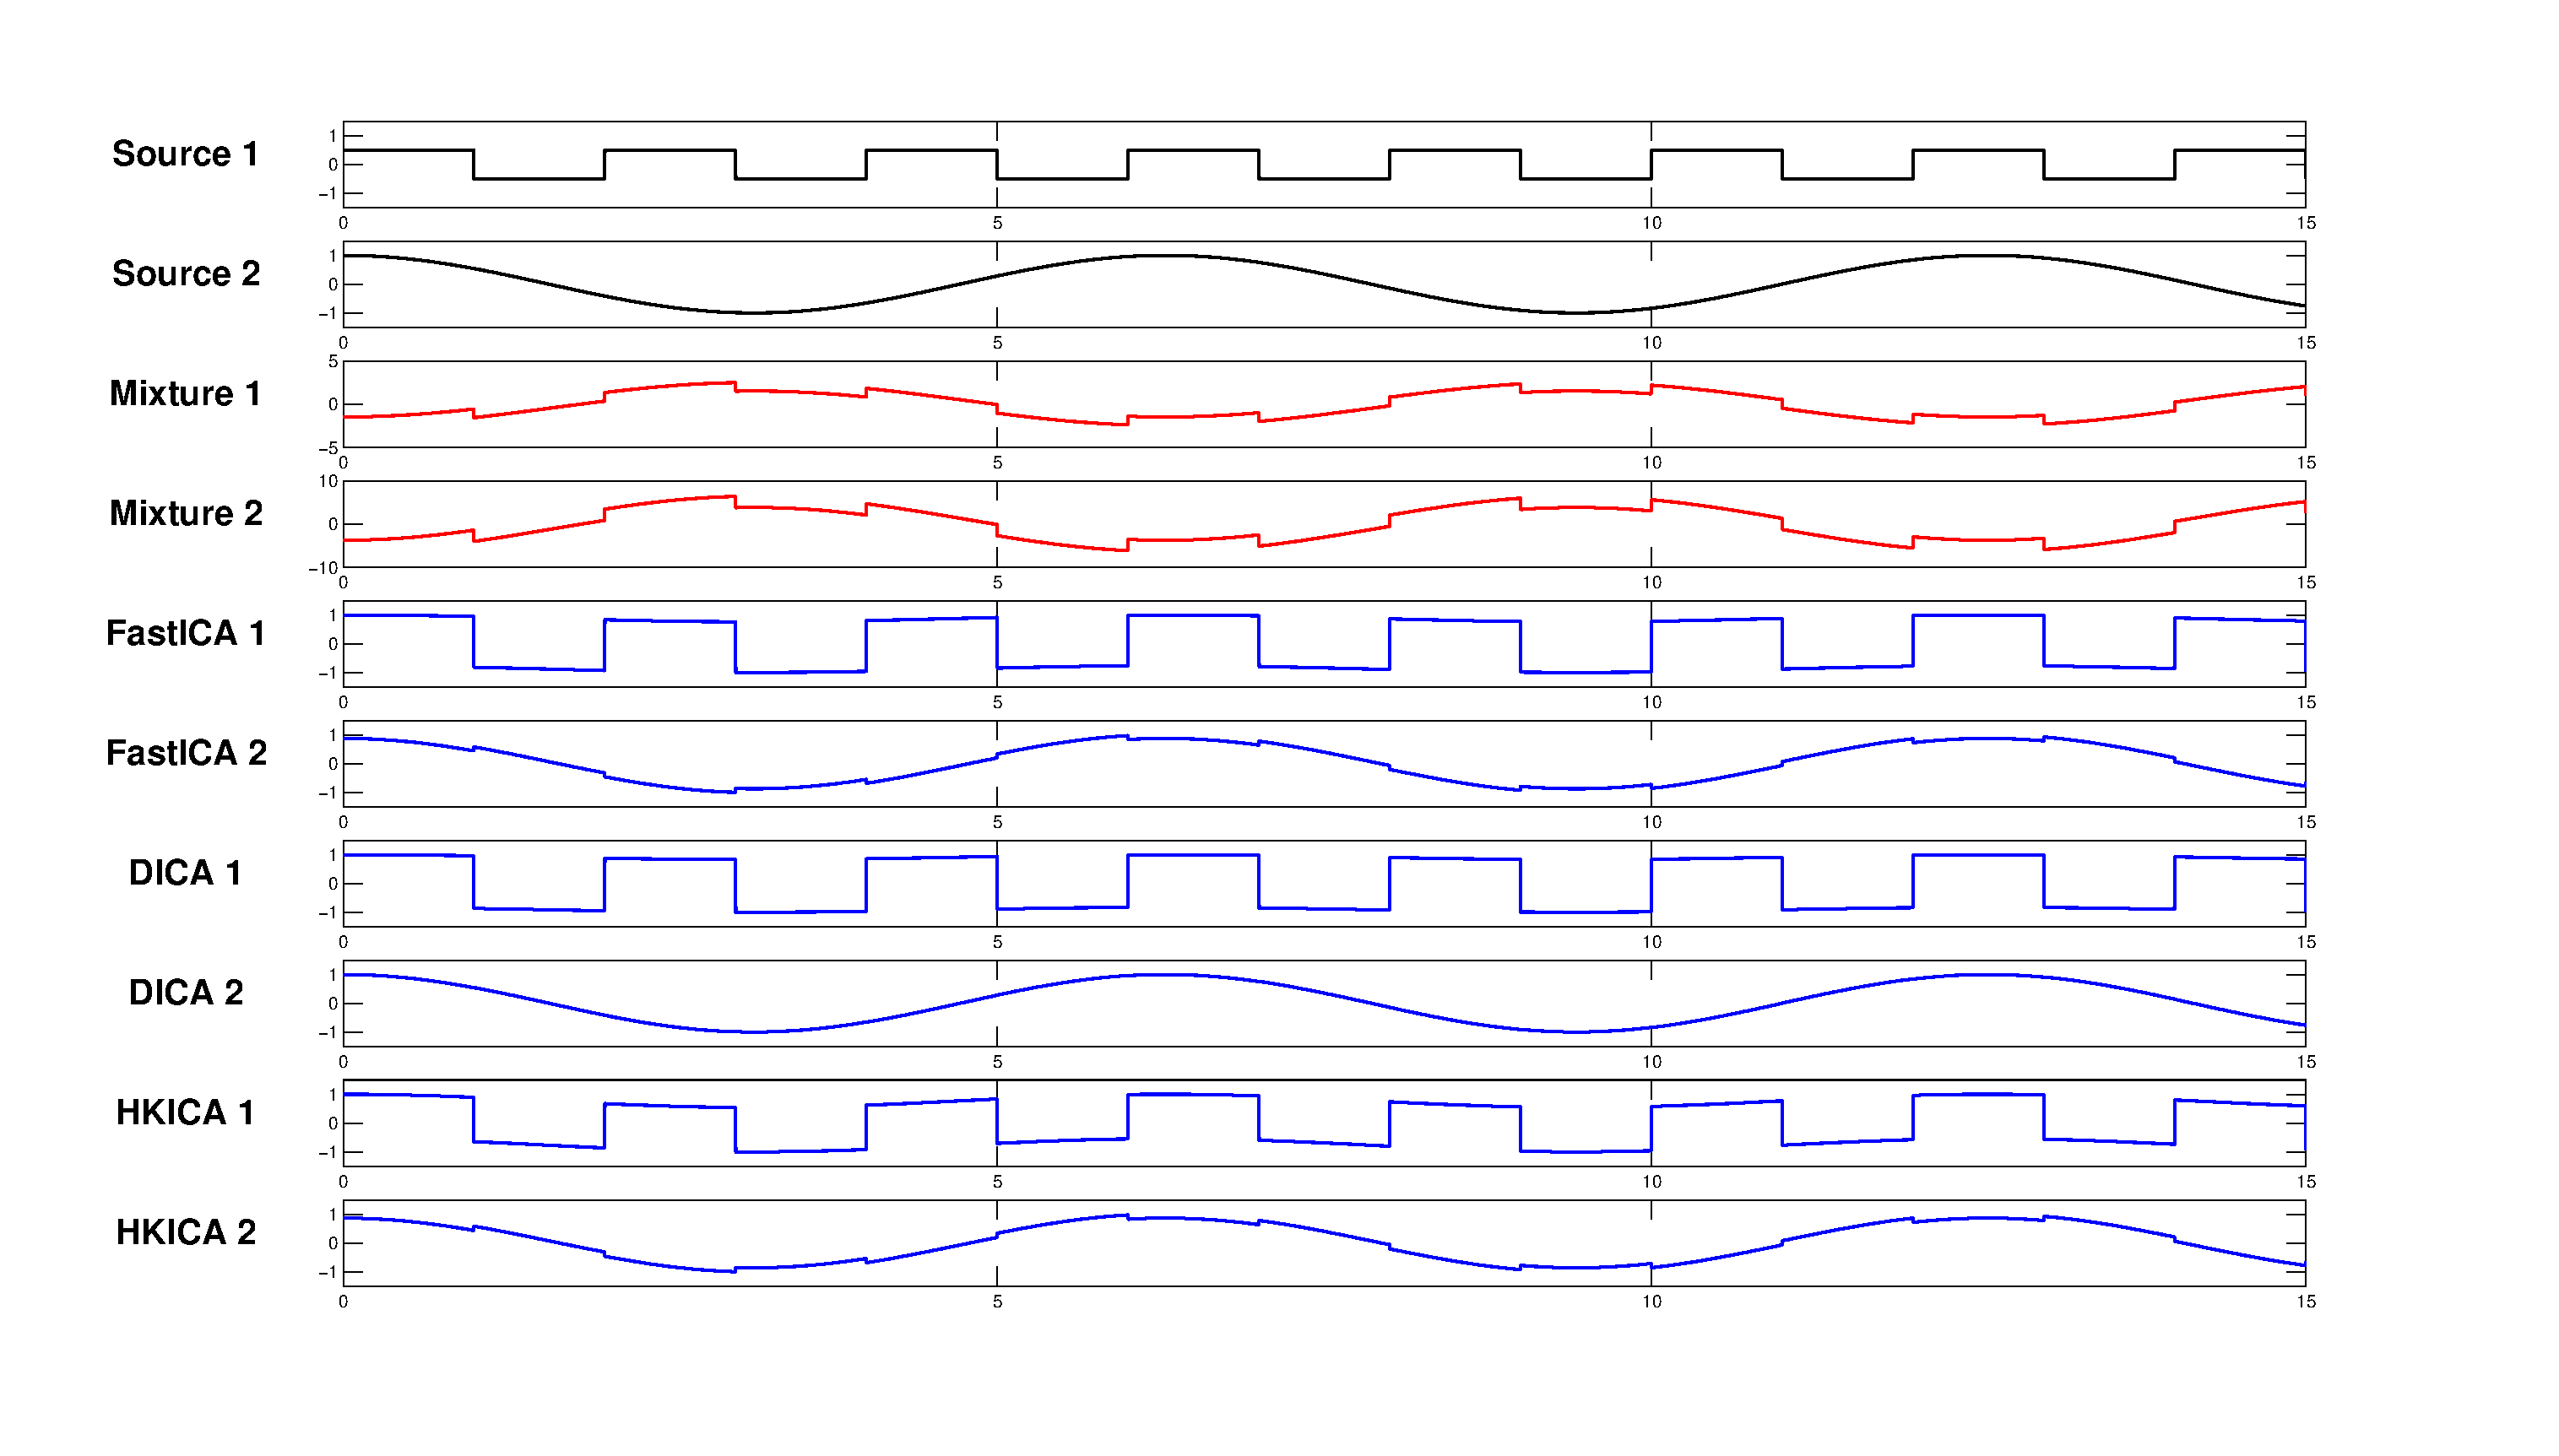
\includegraphics[width = 0.8\textwidth]{demo}
				%\caption*{Behavior of various ICA methods}
			\end{figure}
			\vspace{-0.5cm} 					
		\end{block}
%		Deterministic signals
		\vspace{0.5ex}

	
		\begin{block}{Classical Definition}
			\centering
			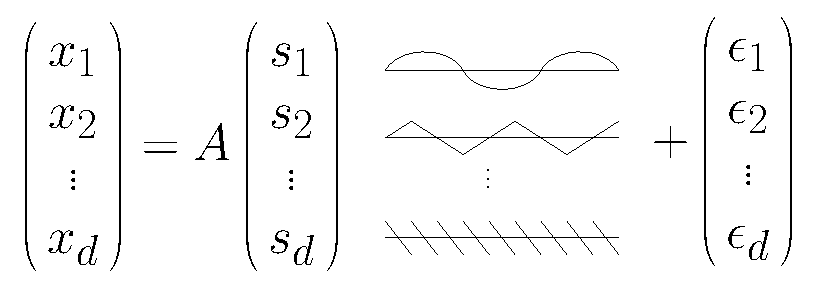
\includegraphics[width=0.7\textwidth]{ICA_model.eps}
			\begin{equation*}
				\label{eq:stoch-ICA}
				X = AS+\epsilon
			\end{equation*}
			\vspace{-1.5cm}
			\begin{itemize}
				\item $S = (S_1,\ldots, S_d)$ non-Gaussian, $\eps \sim \mathcal{N}(0,\Sigma)$ Gaussian random variables.
				\item Goal: Given $T$ independent observations $X(1), \ldots, X(T) \sim X$, reconstruct $A$ up to scaling and permutation.
\item Assumptions:
                          \begin{itemize}
				\item $S_1(t),\ldots, S_d(t)$, $\eps_1(t), \ldots, \eps_d(t)$ are mutually independent for any $t$.
				\item $A$ is non-singular
                                  (for simplicity). 
                             \end{itemize}
				\item Applications:
				\begin{itemize}
						\item Optical imaging;
						\item Communications;
						\item Neuroscience, EEG, etc.
				\end{itemize}				
			\end{itemize}	
\end{block}


			
		\begin{block}{Previous works}
		\vspace{-0.5cm}
			\begin{itemize}
				\item The literature in ICA is vast, but only for stochastic setting.
				\begin{itemize}
					\item Fast ICA \citep{hyvarinen1999fast}; Moment methods:
					Arora et al.'s method \citep{arora2012provable},
					Hsu and Kakade's method \citep{hsu2013learning} (HKICA), 
					Fourier PCA \citep{goyal2014fourier} (FPCA).	
				\end{itemize}
				\item No or weak theoretical guarantees / free parameters. % / depends of unspecified parameters.
			\end{itemize}
		\end{block}

	\end{column}
%------------------------------------------------------------------------------
% The second column
%------------------------------------------------------------------------------	
	\begin{column}{0.01\textwidth}
	\end{column}
	
	\begin{column}{.24\textwidth}% the right size for a 3-column layout
		\begin{block}{Deterministic?}
			\begin{itemize}
				\item It is well known that ICA works well on unmixing deterministic signals!
				\item All deterministic sequences satisfy the independence assumption $\dots$
				\item Can some ICA method unmix \alert{any} deterministic signals?
			\end{itemize}
			\begin{center}
				{\large Not really!}
			\end{center}
			
			\vspace{1cm}
			\begin{tcolorbox}[title = \vspace{0.4cm}\textbf{\large Our Contributions} \vspace{0.4cm}, title filled, width = 0.9\textwidth, colback = uofagreen!10, colframe = red]
			\begin{itemize}
			\vspace{0.5cm}
			\item[$\diamondsuit$] Extend ICA to a non-stochastic setting that covers
			\begin{itemize}
			\item[--] the classical stochastic setting;
			\item[--] Markov sources;
			\item[--] deterministic source signals.
			\end{itemize} 
			\vspace{1cm}
			\item[$\diamondsuit$] Develop, \emph{for the first time in the literature}, ICA methods that have
				\begin{itemize}
					\item[--] $\mathrm{poly}(T,d)$ runtime;
					\item[--] $\mathrm{poly}(D_4)$ accuracy;%
					\footnote{For the definition of $D_4$ see below.}
					\item[--] no free parameters
				\end{itemize}
			\end{itemize}		
			\end{tcolorbox}
		\end{block}
		\vspace{0.5ex}
		\begin{block}{Non-stochastic settings}
			\begin{itemize}
				\item The source signals are a function of time: $s:[T] \to [-C,C]^d$.
				\item Empirical distribution induced by function $s$:
				\[
					\nu_t^{(s)}(B)=\tfrac{1}{t}|\{\tau \in [t]: s(\tau) \in B\}|.
				\]
				\item Independence measure of the sources:
				Let $\mu$ be a product measure and let
				\[
				D_4(\nu_T^{(s)},\mu) = \sup_{f\in\mathcal{F}} \Big|\int f(s)d\nu_T^{(s)} - \int f(s)d\mu(s)\Big|,
				\]
				where $\mathcal{F}$ is the set of all monomials up to degree $4$.
			\end{itemize}
		\end{block}
	\end{column}
%------------------------------------------------------------------------------
% The third column
%------------------------------------------------------------------------------
	\begin{column}{0.01\textwidth}
	\end{column}
	\begin{column} {.24\textwidth}
		\begin{block}{Result}
			$\exists$ method to estimate $A$ from $x(t)=A s(t)$, $t=1,\dots,T$ s.t.:
			\begin{itemize}
				\item The computational complexity is $O(d^3 T)$;
				\item With high probability there exists a permutation $\pi$ and constants $\{c_1,\ldots,c_d\}$, such that for all $1\le k\le d$, 
				\[\| c_k\hat{A}_{\pi(k)} - A_k\|_2 \le g(T),\]
				given that 
				\begin{itemize}
					\item[-]  $T$ is large enough;
					\item[-]  there exists a product measure $\mu$ such that $D_4(\nu_T^{(s)},\mu)$ is small enough ($s$ independent enough).
				\end{itemize}
				\item Here $g(T)$ is a function of $D_4(\nu_T^{(s)},\mu)$. In the classic stochastic setting, $g(T) = O(\frac{1}{\sqrt{T}})$.
			\end{itemize}
		\end{block}
		\vspace{0.5ex}
		\begin{block}{Hsu and Kakade's method (HKICA)}
			\begin{figure}
			\begin{algorithmic}[1]
				\STATE Let $f(\eta) = \EEp{(\eta^{\top}x)^4} - 3 \EEp{(\eta^{\top}x)^2}^2$.
				\STATE  Choose $\phi$ and $\psi$. (How?)
				\STATE Let $T(\phi) = \nabla^2 f(\phi)$. Then 
					\[T(\phi) = AK \triangle\left( (\sigma_1,\ldots,  \sigma_d)\right)A^{\top},
					\]
					where $\sigma_i = \left(\phi^{\top}A_i\right)^2$ and $K$ is some diagonal matrix.
				\STATE Let $M = T(\phi)(T(\psi))^{-1}$. Then 
					\[M = A \triangle \left( \lambda_1, \ldots, \lambda_d \right) A^{-1},
					\]
					where $\lambda_i = \left(\frac{\phi^{\top}A_i}{\psi^{\top}A_i}\right)^2$.
				\STATE Do an eigen-decomposition of $M$ to recover $A$, assuming all $\lambda_i$'s are distinct.
			\end{algorithmic}
			\end{figure}
			\vspace{1cm}
			{\it\large{Problem: Minimal gap of the eigenvalues.}}
			\begin{itemize}
				\item Theoretical analysis shows that the performance depends on 
					\[
					\gamma_A = \min_{i\neq j} \left\vert \lambda_i - \lambda_j\right \vert.
					\]
				\vspace{-1cm}
				\item $\gamma_A$ is not yet well understood.
			\end{itemize}
		\end{block}
	\end{column}
%------------------------------------------------------------------------------
% The fourth column
%------------------------------------------------------------------------------	

	\begin{column}{0.01\textwidth}
	\end{column}
	\begin{column}{0.24\textwidth}
		\begin{block}{Our method: Deterministic ICA (DICA)}		
			\begin{figure}
			\begin{algorithmic}[1]
				\STATE Sample $\psi$, $\phi_1$, and $\phi_2$ independently from standard normal distribution.
				\STATE Calculate $\nabla^2 f(\psi)$ and $B$ such that $\nabla^2 f(\psi) = BB^{\top}$.
				\STATE Calculate $T(\phi_1) = \nabla^2 f(B^{-\top}\phi_1)$ and $T(\phi_2) = \nabla^2 f(B^{-\top}\phi_2)$.
				\STATE Calculate $M = T(\phi_1)(T(\phi_2))^{-1}$.
					\[
					M = R \left( \tilde{\lambda}_1, \ldots, \tilde{\lambda}_d \right)R^{\top},
					\]
					where $\tilde{\lambda}_i = \left(\frac{\phi_1^{\top}R_i}{\phi_2^{\top}R_i}\right)^2$ and $R$ is some orthonormal matrix.
				\STATE Do an eigen-decomposition of $M$ to recover $R$.
				\STATE Return $\hat{A} = BR$ as an estimation of $A$. 
			\end{algorithmic}
			\end{figure}
			\begin{itemize}
				\item $\tilde{\lambda}$ (and its minimal gap) is now independent of $A$, and easier to analyze.
				\item Simulation results are provided in the paper.
			\end{itemize}
		\end{block}
		\vspace{0.5ex}
		\begin{block}{Recursive version}
			\begin{itemize}
				\item Based on the idea of Vempala et al. \citep{vempala2014max};
				\item Changes the dependence on the minimal gap to the maximal gap by taking a recursive procedure;
				\item Helps reduce the sample complexity;
				\item See the paper for details.
			\end{itemize}
		\end{block}
		\begin{block}{References}
			\scriptsize
			\bibliographystyle{plain}
			\bibliography{DICA}
		\end{block}			
	\end{column}
		
	\begin{column}{0.01\textwidth}
	\end{column}
\end{columns}
 
\end{frame}

\end{document}
